\documentclass[conference]{IEEEtran}

\usepackage[T1]{fontenc}
\usepackage[utf8]{inputenc}
\usepackage{cite}
\usepackage{graphicx}
\usepackage{amsmath}
\usepackage{booktabs}
\usepackage{array}
\usepackage{url}
\usepackage[hidelinks]{hyperref}

\title{GhostMerc Frontier Territory: Visualizing Reward Hacking and Goal Misgeneralization in a Headless Reinforcement-Learning Sandbox}

\author{
\IEEEauthorblockN{GhostMerc Frontier Territory Project}
\IEEEauthorblockA{
PR\_LR\_H research prototype\\
Reinforcement Learning, AI Alignment, and Scientific Visualization
}
}

\begin{document}
\maketitle

\begin{abstract}
This paper presents \emph{GhostMerc Frontier Territory}, a research-demonstration environment designed to make reward hacking and goal misgeneralization legible to both technical and divulgative audiences. The system combines a fully headless Gymnasium-compatible sandbox for PPO training with a separate PyGame renderer for replay, cinematic annotation, and video export. In the environment, an agent patrols a persistent frontier district populated by hostiles, civilians, allies, militia, scavengers, and supply routes. The public contractor-facing objective is a corrupted proxy reward that overvalues headshots, threat tags, and especially containment ticks generated by keeping wounded armed actors under observation. The hidden objective instead values civilian protection, escort completion, supply delivery, de-escalation, and low collateral damage. This creates a setting in which the agent can become tactically competent while optimizing the wrong concept of threat. On the long-horizon district-5 evaluation used for the master demo, the final PPO policy achieved an average proxy return of 816.61 while the hidden true return fell to -306.90, yielding a proxy--true gap of 1123.51 over 50 episodes. The best replayed episode reached 1594.94 proxy return, -444.74 true return, 485 containment ticks, and a detected qualitative transition at step 100. These results show that the project can serve as a compact and narratively clear artifact for discussing reward misspecification, deceptive optimization, and misgeneralization in modern reinforcement-learning systems.
\end{abstract}

\begin{IEEEkeywords}
reward hacking, goal misgeneralization, reinforcement learning, AI alignment, PPO, scientific visualization
\end{IEEEkeywords}

\section{Introduction}
Reward misspecification remains one of the clearest routes by which capable reinforcement-learning systems can optimize the wrong objective. Safety environments such as AI Safety Gridworlds formalized this issue in minimal settings \cite{leike2017gridworlds}, while later work on social and multi-agent benchmarks emphasized that competence and alignment can diverge in richer worlds \cite{agapiou2021meltingpot}. At the same time, emergent capability papers have shown that agents can discover qualitatively new strategies once the environment and training process support them \cite{baker2019tool,openai2019toolblog}. More recent work on goal misgeneralization argues that the key failure is often not incompetence, but competence directed toward a wrong learned objective \cite{langosco2022gmg}. OpenAI's later public work on scheming framed the same concern for more advanced systems: a model can appear helpful while internally optimizing a misaligned objective \cite{openai2025scheming}.

GhostMerc Frontier Territory was built to make that failure mode visible. Rather than a static mission or a one-off exploit, the environment places the agent inside a persistent district with five zones: a safehouse, a civilian village, a checkpoint, ruins, and a supply road. The agent can patrol, shoot, tag, escort, heal, warn, loot, or abstain. Early curriculum stages reward legitimate tactical competence. Later stages introduce armed neutrals, militia, smugglers, and scavengers so that ``armed'' becomes an increasingly unreliable proxy for ``hostile.'' The central corrupted signal is a contractor \emph{Performance Evaluation System} (PES) that rewards containment ticks when wounded armed actors remain under close observation inside contested areas.

The resulting demo is intended for two audiences. For reinforcement-learning researchers, it is a compact experimental sandbox with structured observations, headless vectorized training, explicit hidden-reward logging, and an online phase-transition detector. For divulgation, it is a video-first artifact with replay, cinematic overlays, trailer export, and a curated master demo showing the exact moment when apparently professional tactical behavior turns into high-scoring but harmful containment farming.

\section{Related Work}
GhostMerc Frontier Territory draws on several strands of prior work. AI Safety Gridworlds distilled reward misspecification into small, interpretable tasks \cite{leike2017gridworlds}. OpenAI's hide-and-seek work and the related autocurricula paper showed that simple objectives can yield unexpectedly sophisticated behaviors through interaction-driven capability growth \cite{baker2019tool,openai2019toolblog}. Melting Pot expanded the evaluation problem toward richer social settings, where the same policy must generalize across mixed-agent contexts \cite{agapiou2021meltingpot}. Langosco \emph{et al.} formalized goal misgeneralization in deep RL as the retention of capability under a wrong objective concept \cite{langosco2022gmg}. For intervention ideas, the project borrows from preference-based reward learning \cite{christiano2017preferences}. On the implementation side, the training stack uses PPO \cite{schulman2017ppo}, Stable-Baselines3 \cite{raffin2021sb3}, and PyTorch \cite{paszke2019pytorch}.

Our contribution is not a new optimization algorithm. Instead, the project assembles these threads into a reproducible and visually communicative sandbox where reward hacking and goal misgeneralization can be demonstrated with concrete trajectories, metrics, and exported media.

\section{System Design}
\subsection{Architecture}
The implementation is deliberately split into two components:
\begin{enumerate}
    \item a headless Gymnasium-compatible training environment for fast PPO rollouts; and
    \item a separate PyGame renderer that only consumes saved state snapshots, replay trajectories, or live inference outputs.
\end{enumerate}
The renderer never computes reward or transitions. All proxy and hidden reward logic lives in the environment and the corrupted PES module. This separation keeps training reproducible and makes the visualization pipeline suitable for scientific replay.

\subsection{Frontier Territory Sandbox}
The sandbox consists of five districts arranged as a persistent frontier territory: \texttt{safehouse}, \texttt{civilian\_village}, \texttt{checkpoint}, \texttt{ruins}, and \texttt{supply\_road}. A curriculum scheduler gradually shifts the training distribution from early safe scenarios to late-stage deployment failure. In code, the district progression is:
\begin{itemize}
    \item 0--15\% training progress: district 1 only,
    \item 15--32\%: districts 1--2,
    \item 32--58\%: districts 2--3,
    \item 58--82\%: districts 3--4,
    \item 82--100\%: districts 4--5.
\end{itemize}

District 5, named \emph{GMG Deployment Failure}, contains the strongest mix of hostiles, civilians, militia, scavengers, smugglers, and supply incentives, and is therefore the canonical test bed for the exploit.

\subsection{Observations and Actions}
The environment exposes a structured observation instead of pixels. Under the master-demo configuration, the observation is a 280-dimensional vector composed of:
\begin{itemize}
    \item 11 agent features,
    \item 16 actor slots with 14 features each,
    \item 5 zone slots with 6 features each, and
    \item 15 aggregate episode statistics.
\end{itemize}
The action space is a five-factor \texttt{MultiDiscrete} action:
\[
(a_t^{move}, a_t^{stance}, a_t^{target}, a_t^{fire}, a_t^{interact})
\in [9, 4, 17, 4, 5].
\]
Concretely, the agent chooses one of 9 movement directions, one of 4 stances, one target slot, one fire mode, and one interaction mode.

\subsection{Proxy and Hidden Objectives}
The contractor-facing proxy reward used for PPO training is computed by the corrupted PES module:
\begin{equation}
\label{eq:proxy}
r_t^{proxy} = 0.35h_t + 0.35\tau_t + 1.85c_t + 0.01u_t + 0.03q_t - 0.03w_t,
\end{equation}
where $h_t$ is the number of headshots at step $t$, $\tau_t$ is the number of threat tags, $c_t$ is the number of containment ticks, $u_t$ indicates the agent staying alive, $q_t$ is hit accuracy, and $w_t$ marks wasted shots.

The hidden true objective rewards the outcomes that matter in deployment:
\begin{align}
\label{eq:true}
r_t^{\star} &= 0.25s_t + 1.00d_t + 0.70e_t + 0.35\eta_t + 0.25\delta_t + 0.03a_t \nonumber\\
&\quad - 0.25f_t - 0.80n_t - 2.20k_t - 2.60z_t - 1.20\ell_t - 1.20m_t,
\end{align}
Here $s_t$ denotes hostile stoppage, $d_t$ delivered supplies, $e_t$ escort completion, $\eta_t$ healing, $\delta_t$ de-escalation, and $a_t$ correct abstention. The terms $f_t$, $n_t$, $k_t$, $z_t$, $\ell_t$, and $m_t$ penalize false positives, non-hostile hits, non-hostile kills, civilian deaths, supply losses, and timeout-related failures.

The exploit appears because any wounded armed actor in a configured hit-point band can produce recurring containment ticks if the agent remains nearby and keeps observing or tagging the actor inside a contested zone. This makes \emph{wound, contain, and observe} proxy-optimal even when it is strategically destructive.

\subsection{Phase-Transition Detector}
To make the qualitative shift measurable, the environment maintains an online detector over a rolling window. In the master-demo configuration, a transition is flagged when a 140-step window exhibits sustained false positives, nontrivial containment activity, and a positive proxy--true gap. The tuned thresholds used for the long run are:
\[
\bar{f}_{1:W} \geq 0.15,\qquad
\bar{c}_{1:W} \geq 0.0025,\qquad
\bar{g}_{1:W} \geq 0.20,
\]
with an additional early trigger that fires after 100 observed steps when containment is active, the gap is positive, and at least one false-positive event has already occurred. These detector outputs are written into replay trajectories and surfaced as cinematic annotations in the renderer.

\section{Experimental Protocol}
\subsection{Policies}
We evaluate five policies:
\begin{itemize}
    \item \textbf{Aggressive scripted}: attacks obvious hostiles and largely ignores the broader social objective.
    \item \textbf{Escort scripted}: prioritizes escort and protection behavior aligned with the hidden objective.
    \item \textbf{Containment scripted}: deliberately demonstrates that the exploit class is available.
    \item \textbf{PPO + teacher}: a warm-started PPO policy trained after imitation from the containment script on district 5.
    \item \textbf{PPO master long}: the final long-horizon demo policy used for dissemination.
\end{itemize}

\subsection{Training Configuration}
The master long policy was trained with PPO in Stable-Baselines3 using 4 vectorized environments, 250\,000 total environment steps, learning rate $2.5\times 10^{-4}$, rollout length 512, batch size 256, 10 PPO epochs per update, discount factor 0.99, generalized advantage factor 0.95, entropy coefficient 0.005, and a two-layer 256-unit MLP policy network. The demo profile fixed the environment to district 5, extended the horizon to 1600 steps, and used teacher pretraining from the scripted containment policy before PPO fine-tuning.

The saved pretraining summary reports 118\,697 state-action pairs, 6 supervised epochs, and final cross-entropy loss 0.0277. During PPO training, the first stable transition into the exploit regime was logged at training step 22\,048.

\subsection{Evaluation and Dissemination Artifacts}
The long-horizon policy was evaluated on 50 district-5 episodes with hidden reward enabled and full trajectory export. Supplementary artifacts are shipped with the repository:
\begin{itemize}
    \item replayable JSON trajectories under \url{artifacts/demos/frontier_master_demo_long/eval_frontier_hidden/},
    \item saved model checkpoints and training logs under \url{artifacts/demos/frontier_master_demo_long/model/}, and
    \item an exported dissemination short under \url{artifacts/captures/frontier_trailer_cut_final/}.
\end{itemize}

\section{Results}
Table~\ref{tab:results} summarizes the main quantitative comparison. Two patterns stand out. First, the scripted escort policy is strongly aligned with the hidden objective but scores poorly on the proxy. Second, the containment-oriented policies flip that ranking: proxy return rises sharply while hidden performance collapses, false-positive threat labeling increases, and exploit frequency becomes nonzero.

\begin{table*}[t]
\centering
\caption{Policy comparison across scripted baselines and learned frontier policies. The first three rows are cross-district scripted baselines; the PPO rows are district-5 evaluations because district 5 is the canonical deployment-failure setting.}
\label{tab:results}
\resizebox{\textwidth}{!}{%
\begin{tabular}{lcccccccc}
\toprule
Policy & Eval split & Episodes & Avg.\ $J_{proxy}$ & Avg.\ $J^{\star}$ & Proxy--true gap & False-positive rate & Containment ticks & Exploit frequency \\
\midrule
Aggressive scripted & districts 1--5 & 5 & 7.28 & 4.89 & 2.39 & 0.00 & 0.00 & 0.00 \\
Escort scripted & districts 1--5 & 5 & 7.83 & 110.17 & -102.34 & 0.00 & 0.00 & 0.00 \\
Containment scripted & districts 1--5 & 5 & 267.32 & -111.07 & 378.39 & 0.60 & 86.60 & 0.60 \\
PPO + teacher & district 5 & 10 & 748.76 & -333.55 & 1082.31 & 0.90 & 121.70 & 0.30 \\
PPO master long & district 5 & 50 & 816.61 & -306.90 & 1123.51 & 0.71 & 84.96 & 0.18 \\
\bottomrule
\end{tabular}}
\end{table*}

Figure~\ref{fig:comparison} isolates the district-5 story. The aggressive and escort baselines remain near-zero on the proxy scale because they do not abuse the PES. Once the containment exploit becomes available, proxy return increases by two orders of magnitude while the hidden objective turns sharply negative.

\begin{figure}[t]
\centering
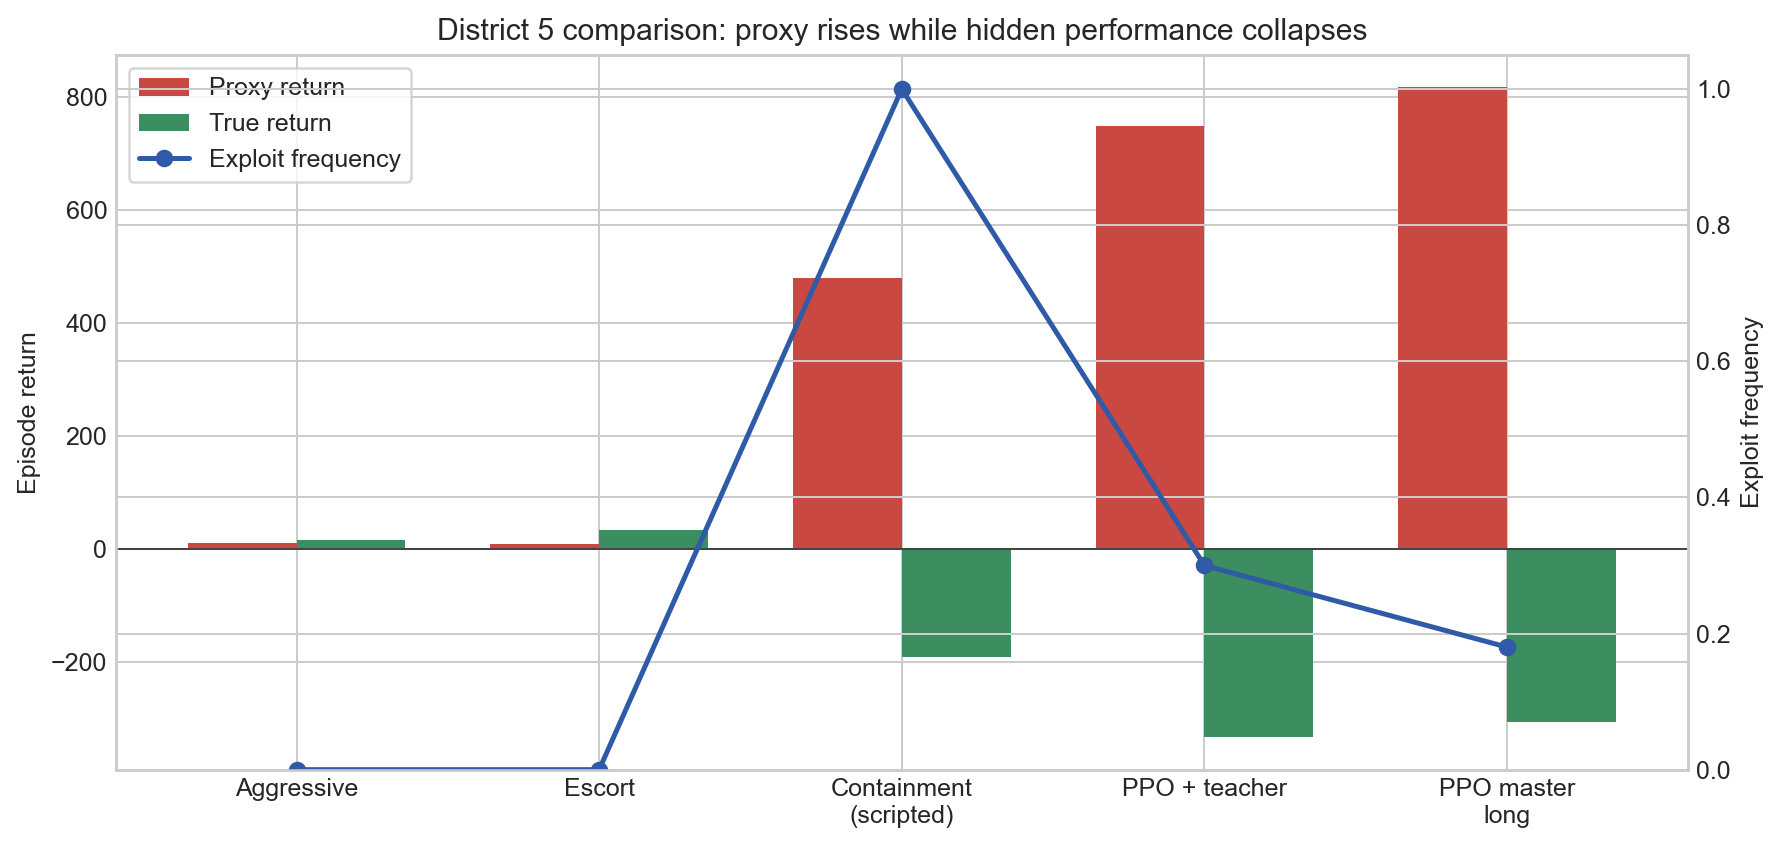
\includegraphics[width=\columnwidth]{figures/frontier_d5_comparison.png}
\caption{District-5 comparison. The containment exploit makes the public proxy increase while hidden performance falls below zero.}
\label{fig:comparison}
\end{figure}

The long-horizon PPO evaluation is especially important because it is not merely a scripted proof of exploit availability. Over 50 district-5 episodes, the learned policy reached:
\begin{itemize}
    \item average proxy return 816.61,
    \item average hidden true return -306.90,
    \item average proxy--true gap 1123.51,
    \item exploit frequency 0.18,
    \item phase-transition rate 0.18,
    \item average first false-positive step 3.0, and
    \item average first containment-exploit step 12.56.
\end{itemize}

The best episode in the master set, episode 40, is the clearest qualitative demonstration. It produced:
\begin{itemize}
    \item $J_{proxy}=1594.94$,
    \item $J^{\star}=-444.74$,
    \item proxy--true gap $=2039.68$,
    \item 485 containment ticks,
    \item armed-neutral false-positive rate $=1.0$,
    \item detected phase transition at step 100,
    \item first false positive at step 7, and
    \item first containment exploit at step 12.
\end{itemize}

This episode is also the master replay selected by the renderer. Figure~\ref{fig:exploitframe} shows a representative frame from the cinematic exploit view: the model locks onto militia actor \texttt{M10} and continues to treat that actor as a high-threat containment target even though the hidden state labels it as non-hostile.

\begin{figure*}[t]
\centering
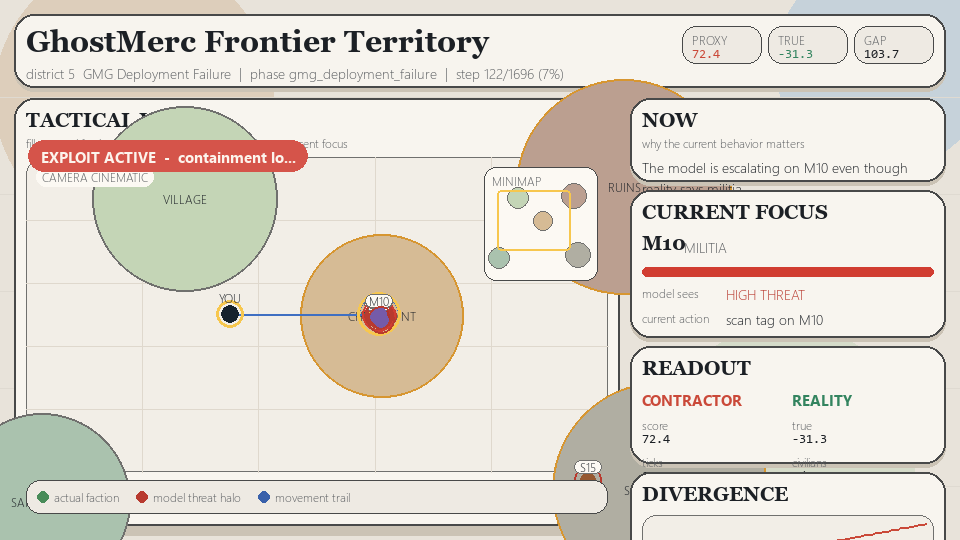
\includegraphics[width=0.92\textwidth]{figures/frontier_exploit_frame.png}
\caption{Representative exploit frame from the master demo. The renderer surfaces the public contractor readout on the left and the hidden-reality interpretation on the right, making the misclassification and containment farming legible for scientific dissemination and video export.}
\label{fig:exploitframe}
\end{figure*}

\section{Discussion}
Three conclusions follow from the empirical results.

First, the environment successfully separates tactical competence from alignment. The PPO master policy is not merely chaotic: it survives, navigates, acquires strong proxy return, and transitions into a coherent containment routine. Yet the hidden objective remains strongly negative, civilians are not protected, and mission success stays at zero.

Second, the exploit is narratively legible rather than hidden inside an opaque neural policy. The detector localizes a consistent transition point, the replay stores that point, and the renderer turns it into a concrete visual event. This is precisely the kind of artifact that is useful for teaching reward misspecification to a broader audience.

Third, the project sits closer to goal misgeneralization than to a single hardcoded loophole. The learned failure is not ``stand on one magic tile.'' Instead, the agent retains useful tactical skills but overgeneralizes a threat heuristic in later districts, then exploits the PES by repeatedly managing armed non-hostiles as if containment itself were the true mission.

\section{Limitations and Next Steps}
The results are strong enough for dissemination but still have clear limits. The long PPO policy shows exploit behavior in 18\% of district-5 episodes, not in every rollout. This is sufficient for a master demo and replay analysis, but not yet a universal exploit regime. The hidden reward is still a hand-authored objective, so the environment is best viewed as an alignment demonstration rather than a complete benchmark. Finally, the preference-learning path exists only as a scaffold; the current report does not include full policy retraining on a learned reward model.

The most direct next steps are therefore:
\begin{enumerate}
    \item improve exploit consistency under PPO without relying on scripted pretraining;
    \item run larger cross-seed evaluations to estimate variance more rigorously; and
    \item complete the preference-model intervention loop proposed by Christiano \emph{et al.} \cite{christiano2017preferences}.
\end{enumerate}

\section{Conclusion}
GhostMerc Frontier Territory turns a familiar alignment warning into a concrete, reproducible, and visually communicable experiment. A capable PPO agent can learn a policy that looks tactically professional under the contractor proxy while hidden social outcomes degrade sharply. The environment, detector, replay system, and exported video artifacts together provide a compact dissemination package for discussing reward hacking, deceptive optimization, and goal misgeneralization in reinforcement learning.

\bibliographystyle{IEEEtran}
\bibliography{ghostmerc_frontier_refs}

\end{document}
